\documentclass{article} % For LaTeX2e
\usepackage{nips15submit_e,times}
\usepackage[colorlinks,linkcolor=red]{hyperref}
\usepackage{url}
\usepackage{amsmath}
\usepackage{graphicx}
\usepackage{float}
\usepackage{bm}
\usepackage{amssymb}
%\documentstyle[nips14submit_09,times,art10]{article} % For LaTeX 2.09


\title{CS499 Homework 7 (First Draft)}


\author{
	Intersteller\thanks{ Use footnote for providing further information
		about author (webpage, alternative address)---\emph{not} for acknowledging
		funding agencies.}
	Department of Computer Science
	Cranberry-Lemon University
	Pittsburgh, PA 15213
}

% The \author macro works with any number of authors. There are two commands
% used to separate the names and addresses of multiple authors: \And and \AND.
%
% Using \And between authors leaves it to \LaTeX{} to determine where to break
% the lines. Using \AND forces a linebreak at that point. So, if \LaTeX{}
% puts 3 of 4 authors names on the first line, and the last on the second
% line, try using \AND instead of \And before the third author name.

\newcommand{\fix}{\marginpar{FIX}}
\newcommand{\new}{\marginpar{NEW}}

%\nipsfinalcopy % Uncomment for camera-ready version

\begin{document}

	\maketitle
	\textbf{Exercise 7.1}\par
	\textbf{(1)}  Since e is in the minimum spanning tree, we split the minimum spanning tree into two components by deleting e. Let the vertices in the two components consist $S$ and $V\backslash S$ respectively. Since there is no circle in a tree, obviously e is the only edge which is good and cross this cut, which means no edge from X crosses this cut. \par
	\textbf{(2)}  Suppose e is not the minimum weight edge crossing this cut, assume there is an edge e' which has less weight and crosses this cut. e' can replace e and consists a spanning tree with less weight. This means e is not in the minimum spanning tree, which means e is not good, which contradicts the condition.\par
	\textbf{Exercies 7.4}
	\begin{figure}[H]
		\centering
		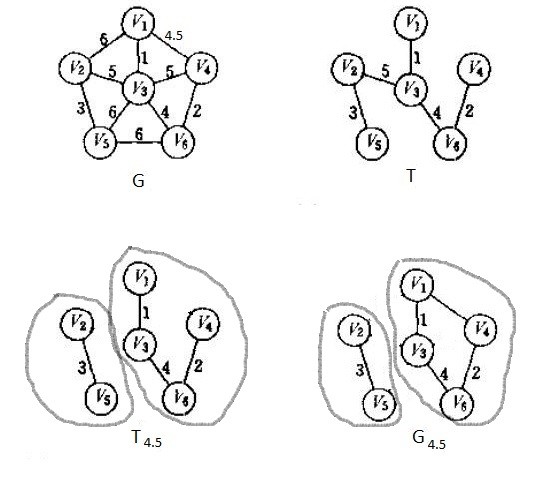
\includegraphics[scale=0.6]{P1.png}
		\caption{}
		\label{fig:1}
	\end{figure}

	\textbf{Exercies 7.5}
	Obviously, if two vertices are connected in $T_c$, they are connected in $G_c$, since $T_c$ is in $G_c$.\\
	Suppose u,v are connected in $G_c$, but not connected in $T_c$. Let two connected components in $T_c$ contain u and v respectively be A and B. Let e be an edge in $G_c$ that connect A and B. Using defination, $w(e)\leq c$. Since A and B are not connected in $T_c$, there must be an edge e' in T that connects A and B, and $w(e')>c$. So, e'>e. Obviously T which contains e' is not the minimum spanning tree, since e' can be replaced by e with less weight. This contradicts the condition. So, if two vertices are connected in $G_c$, they are connected in $T_c$.\par 


	\textbf{Exercise 7.8}\par
    As the picture shows , for $\forall c,m_c(T)=m_c(T\prime)$.
    \begin{figure}[H]
		\centering
		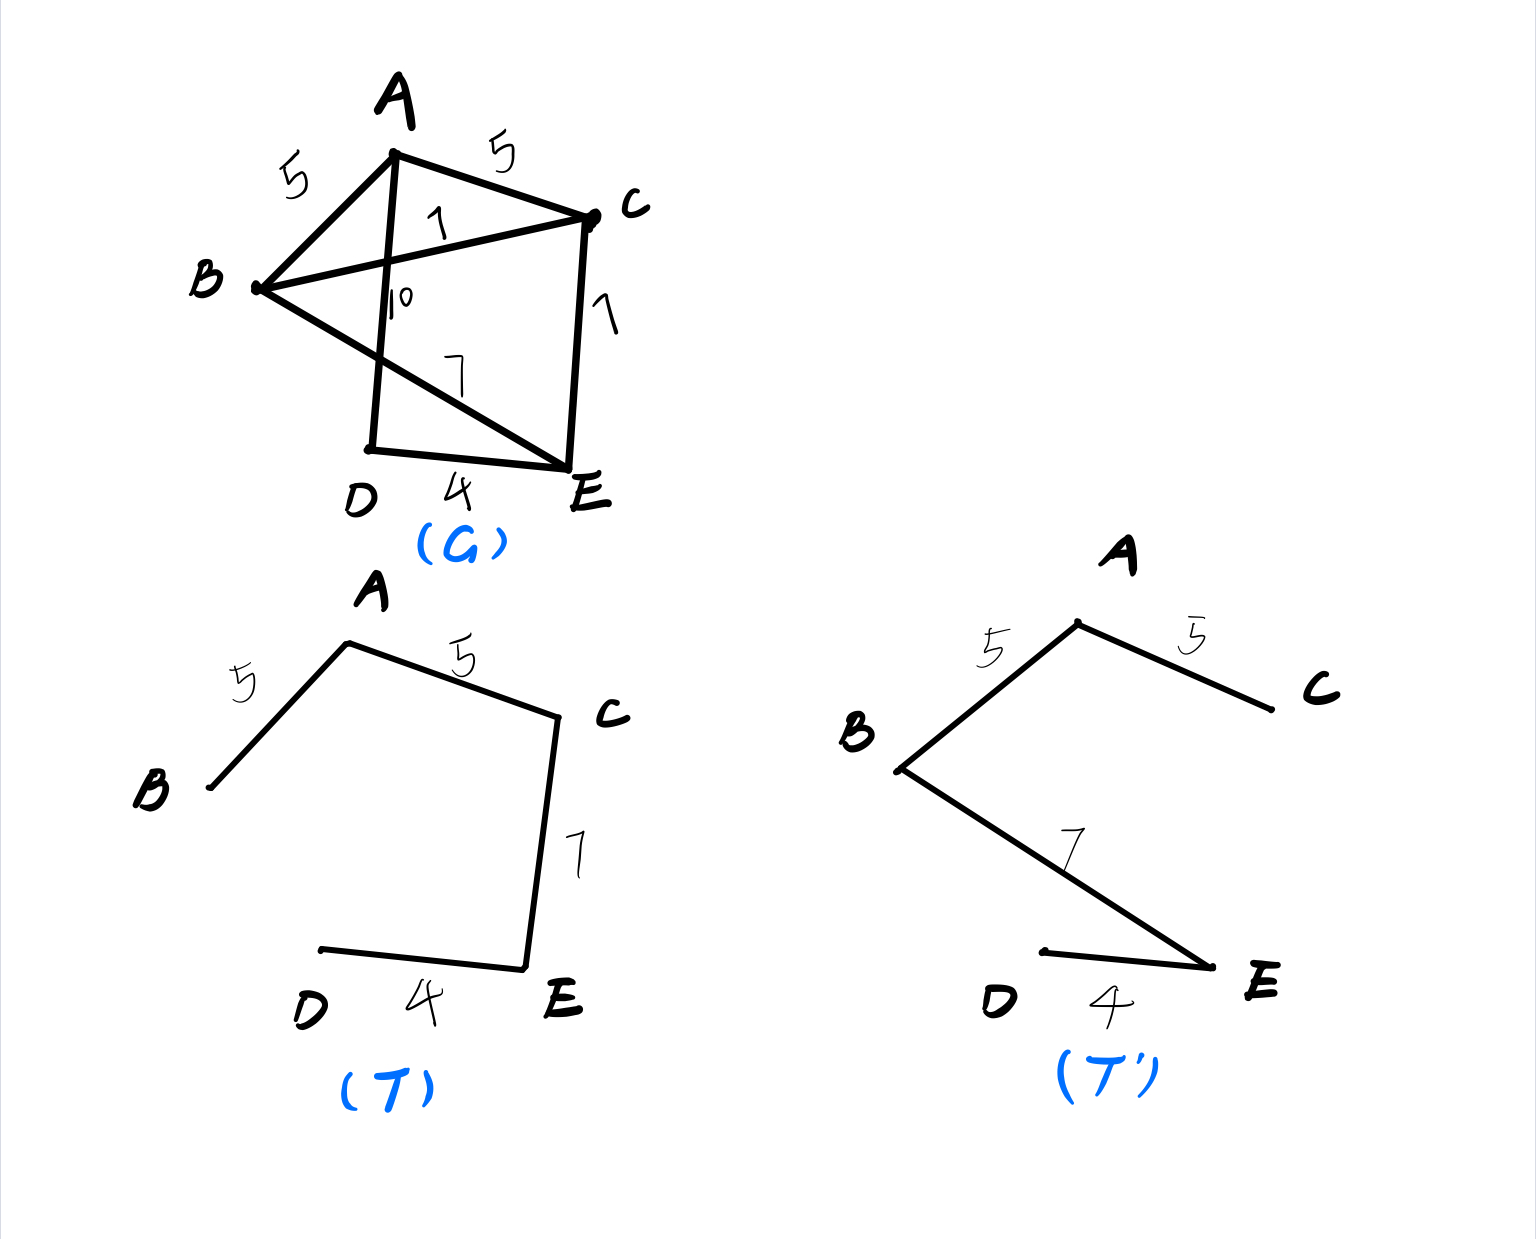
\includegraphics[scale=0.3]{p3.jpg}
		\caption{}
		\label{fig:2}
	\end{figure}

  

	\textbf{Exercise 7.9}\par
    Sort by the weight of $T's$ edges and $T\prime's$ edges , we have $(a1,a2,a3,\cdots,a_{n-1})$ , $(b1,b2,b3,\cdots,b_{n-1})$ . Suppose $a_i\ne b_i$ , $\forall k<i,a_k=b_k$ and $w(a_i)\geq w(b_i)$ , there are two situations:\par
    $(1)$ edge $b_i$ exists in the $T$ , then we can find $j(j>i)$ and $a_j=b_i$ . Because $w(b_i)=w(a_j)\geq w(a_i)\geq w(b_i) , w(a_i)=w(b_i)=w(a_j) . $So we can exchange $a_i$ and $a_j$ and new sequence is still ordered . $T's$ and $T\prime's$ i position is the same edge.\par
    $(2)$ edge $b_i$ doesn't exist in the $T$ , then we add $b_i$ to $T$ to form a cycle . Because $T$ is a minimum spanning tree , $w$(edge in the cycle)$\leq w(b_i)$ . And we can find $a_j$($j>i$ and $a_j$ doesn't exist in the $T\prime$ and $a_j$ in the cycle) . Because $w(b_i)\geq w(a_j)\geq w(a_i) \geq w(b_i),w(b_i)=w(a_i)=w(a_j).$ So we can change $a_j$ with $b_i$ . Turn to the situation $(1)$.\par
    So we know the ordered edge weight list of any two minimum spanning trees is the same.\par
    Obviously, $m_c(T)=m_c(T\prime).$

	
	\textbf{Exercise 7.10}\par
	Suppose there are two minimum spanning tree , sort by the weight of $T's$ edges and $T\prime's$ edges , we have$(a1,a2,a3,\cdots,a_{n-1})$ , $(b1,b2,b3,\cdots,b_{n-1})$.$\exists i,a_i \ne b_i$,based on the $7.9$,the ordered edge weight list of any two minimum spanning trees is the same,so $w(a_i)=w(b_i)$.But no two edges of $G$ have the same weight , so there is contradiction . So $G$ has exactly one minimum spanning tree!
	
	\textbf{Exercise 7.11}\par
	
A function with a core of size 1 forms a rooted tree (the element in core is the root). There are $n^{n-2}$ trees we can form. For each tree we can choose any one of $n$ nodes to be the root, so there are totally $n \cdot n^{n-2}=n^{n-1}$ different rooted trees, which means there are $n^{n-1}$ such functions.\par
	\textbf{Exercise 7.12}\par

A function with a core of size 2 forms a tree whose head and but are connected. There are $n^{n-2}$ trees we can form. For each tree we can choose any one of $n-1$ edges to be the edge connecting the head and the but. Since the head's order number is smaller than but's,once we choose an edge, the head and but are fixed.So there are totally $(n-1) \cdot n^{n-2}=(n-1)\cdot n^{n-2}$ different rooted trees, which means there are $(n-1)\cdot n^{n-2}$ such functions.\par
    
    	\textbf{Exercise 7.13}\par
  	\begin{figure}[H]
  	\centering
  	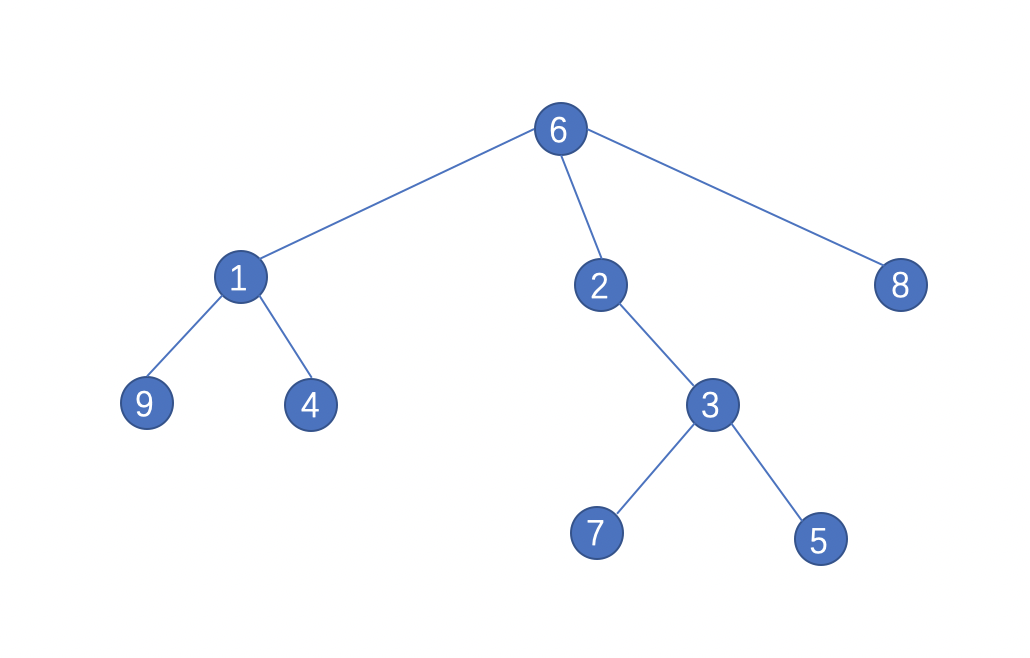
\includegraphics[scale=0.6]{713.png}
  	\caption{}
  	\label{}
  	\end{figure}
	 
	\textbf{Exercise 7.14}\par
	The degree of vertex $i$ is equal to appearance times of $i$ in \textbf{p} plus one.\par
	The nodes that don't appear in \textbf{p} are the leaves of $T$.\par
	  
	\textbf{Exercise 7.15}\par
	1.\par
  	\begin{figure}[H]
  	\centering
  	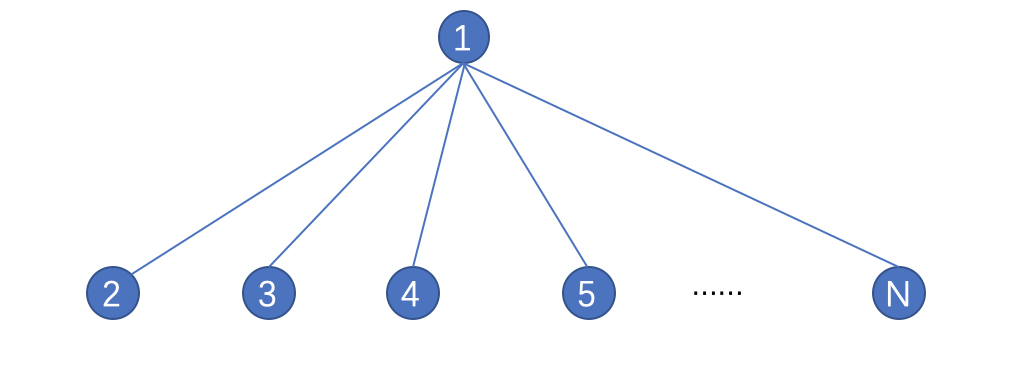
\includegraphics[scale=0.6]{7151.png}
  	\caption{}
  	\label{}
  	\end{figure}
	2.\par
  	\begin{figure}[H]
  	\centering
  	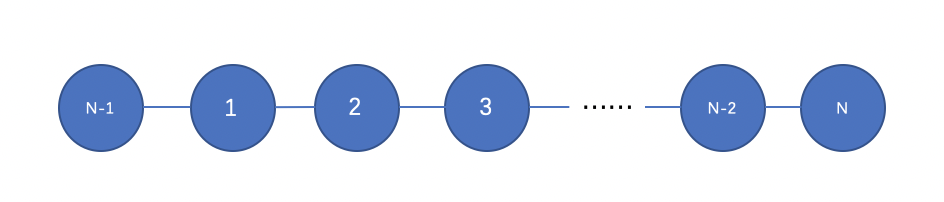
\includegraphics[scale=0.6]{7152.png}
  	\caption{}
  	\label{}
  	\end{figure}
	3.\par
  	\begin{figure}[H]
  	\centering
  	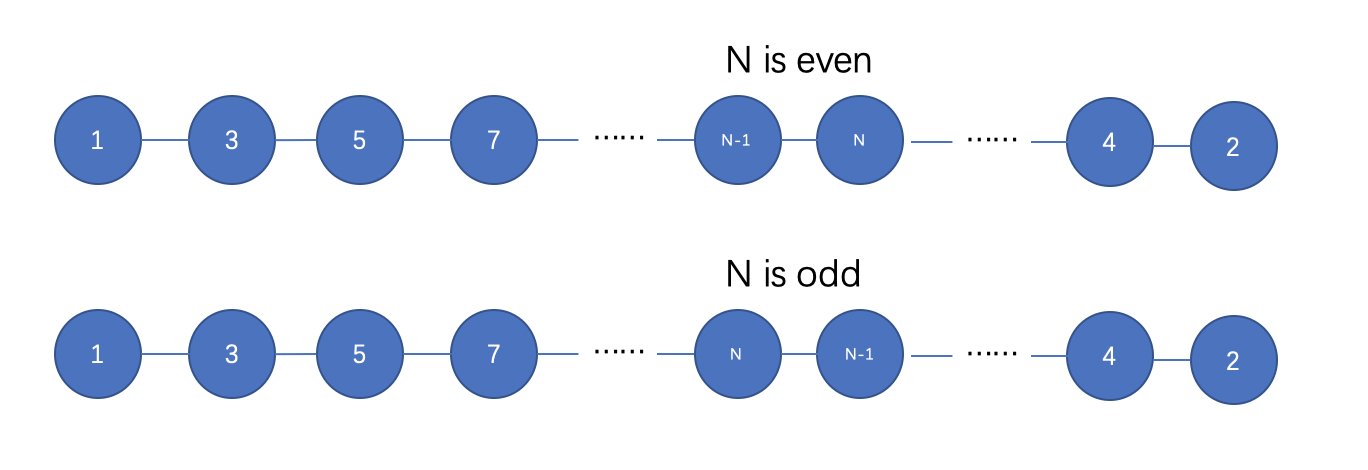
\includegraphics[scale=0.6]{7153.png}
  	\caption{}
  	\label{}
  	\end{figure}
	4.\par
  	\begin{figure}[H]
  	\centering
  	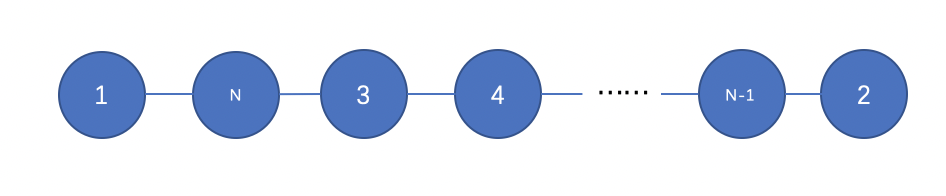
\includegraphics[scale=0.6]{7154.png}
  	\caption{}
  	\label{}
  	\end{figure}
	5.\par
  	\begin{figure}[H]
  	\centering
  	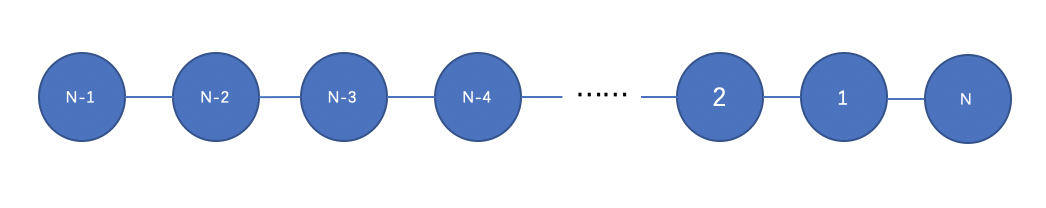
\includegraphics[scale=0.6]{7155.png}
  	\caption{}
  	\label{}
  	\end{figure}
	6.\par
  	\begin{figure}[H]
  	\centering
  	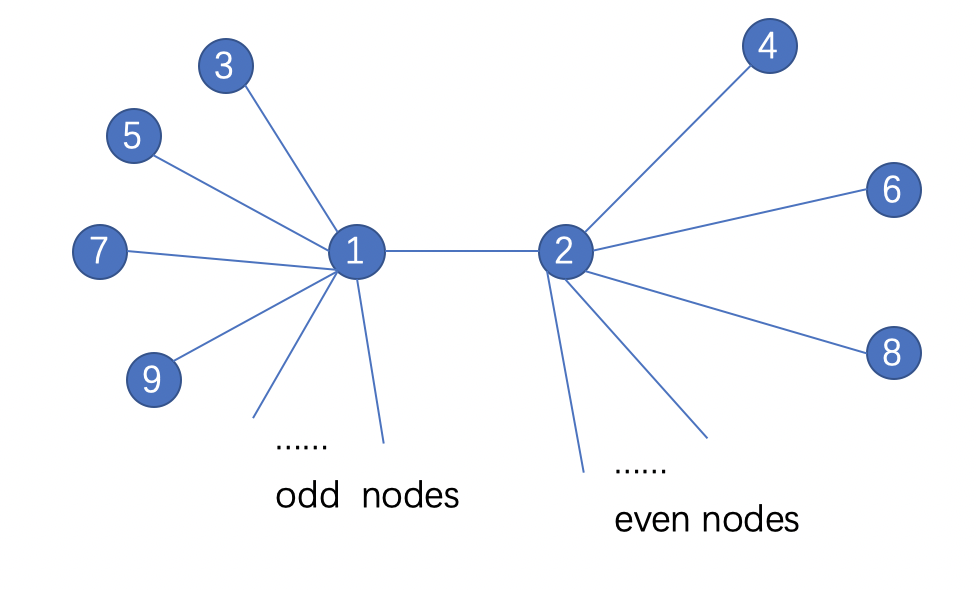
\includegraphics[scale=0.6]{7156.png}
  	\caption{}
  	\label{}
  	\end{figure}
	\textbf{Exercise 7.16}\par
  	\begin{figure}[H]
  	\centering
  	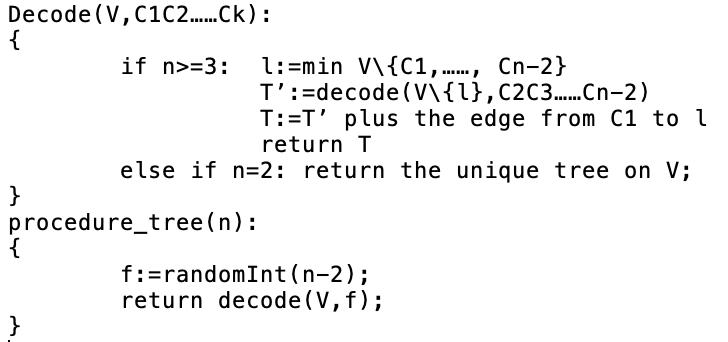
\includegraphics[scale=0.8]{7161.png}
  	\caption{}
  	\label{}
  	\end{figure}
	\textbf{Exercise 7.17}\par
	Pr$[$u is a leaf in $T]=(\frac{n-1}{n})^{n-2}$\par
	E$[$number of leaves$]=n\times(1-\frac{1}{n})^{n}\times (\frac{n}{n-1})^2$\par
	As $n\rightarrow\infty$, $(1-\frac{1}{n})^{n}\rightarrow\frac{1}{e}$,  $(\frac{n}{n-1})^2\rightarrow1$\par
	Thus E$[$number of leaves$]=\frac{n}{e}$\par
	\textbf{Exercise 7.18}\par
	$u$ has degree $2$ means $u$ appear one time in code.\par
	Pr$[u$ has degree $2]=(n-2)\times\frac{1}{n}\times(\frac{n-1}{n})^{n-3}=\frac{(n-2)(n-1)^{n-3}}{n^{n-2}}$\par
	\textbf{Question:}\par
	\textbf{1.}  In Exercise 7.11 \& 7.12, how can we compute the number of functions with a core of size $k$? $(1\leq k\leq n)$



\end{document}
	

